\documentclass[11pt]{article}
\usepackage{graphicx}

\begin{document}
	
	\begin{center}
		Assignment No 1
	\end{center}•
	
	\noindent
	Aim:\\Implement a lexical analyzer for a sample language using LEX.\\
	
	\noindent
	Objective:\\
	\begin{enumerate}
		\item To understand basic syntax of LEX specifications,built-in functions and variables.
		\item To design lexical analyser for sample language
	\end{enumerate}•
	
	\noindent
	Software:\\
	\begin{enumerate}
		\item Linux Operating System
		\item GCCcompiler
	\end{enumerate}•
	
	\noindent
	MATHEMATICALMODEL:\\
	
	\noindent
	Consider a set S consisting of all the elements related to a program.The mathematical model is given as below,\\
	S={s,e,X,Y,Fme,DD,NDD,Memshared}Where,\\
	s=Initial State\\
	e=End State\\
	X=sample language\\
	Y={token,symboltable}\\
	Fme=Algorithm/Functionusedinprogram.foreg.{yylex}DD=Deterministic Data\\
	NDD=Nondeterministic Data\\
	Memshared=Memory shared by processor.\\
	
	\noindent
	THEORY\\
	Introduction:\\
	THEORY:\\
	Introduction:\\
	
	\noindent
	Lexical tool for building lexical analyzer so lexers. A lexer takes an arbitrary input stream and tokenizes it, i.e. ,divides it up in to lexical tokens. This tokenized output can then be processed further, usually by yacc, or it can be the “endproduct”.\\
	
	\noindent
	Lex Specifications:\\
	A Lex program has the following form:\\
	
	\%{\\
		$<$C global variables, prototypes, comments$>$\\
		\%}\\
	
	[DEFINITION SECTION]
	
	\%\%\\
	
	\%\%\\
	
	$<$Cauxiliary  subroutines$>$
	
	
	\%\%\\
	$[$RULESSECTION$]$\\
	
	$<$pattern$>${$<$action to take when matched$>$}
	$<$pattern$>${$<$action to take when matched$>$}
	\%\%
	
	LEX Regular Expressions:\\
	
	\begin{center}
		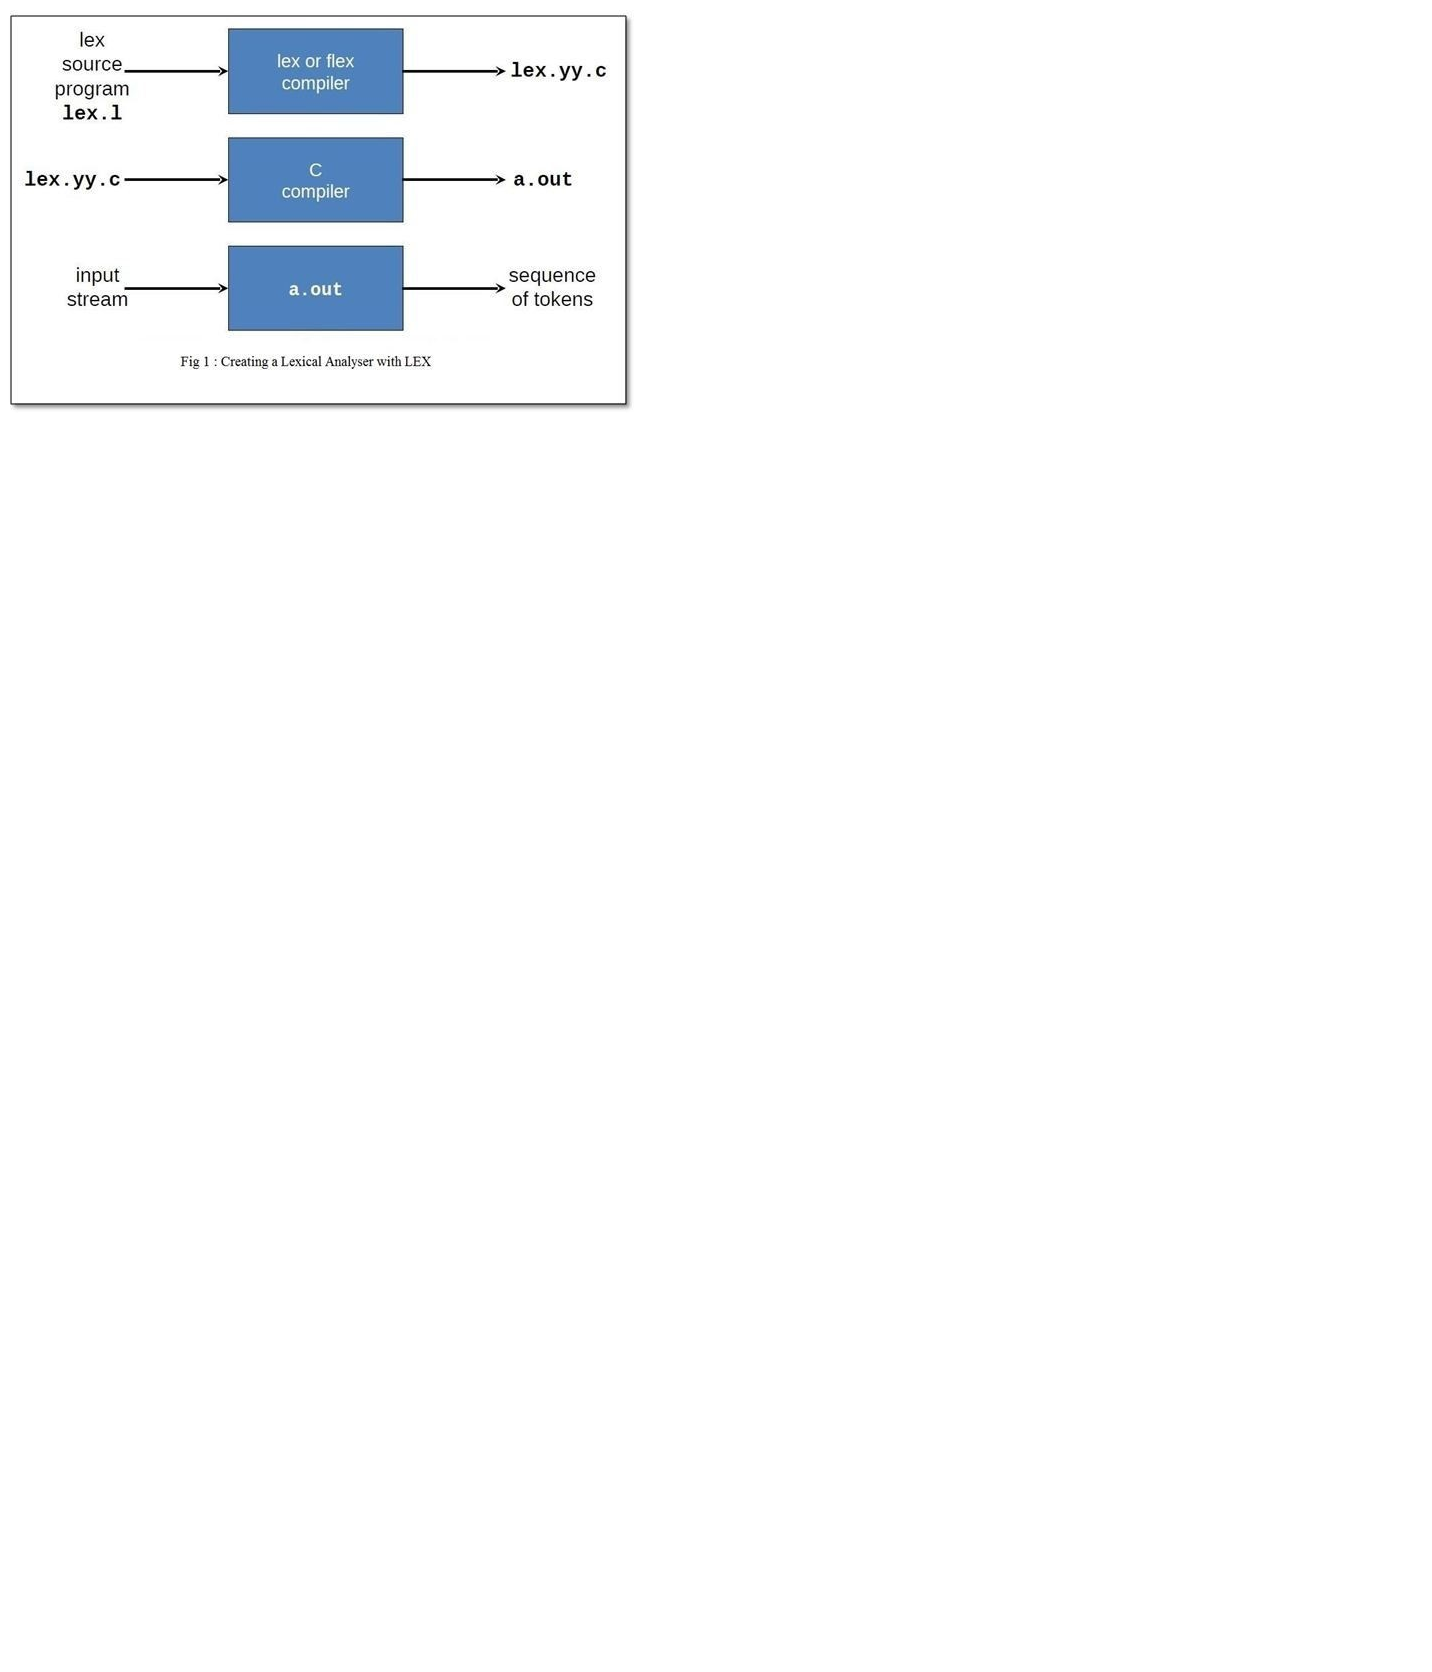
\includegraphics{temp.png}
		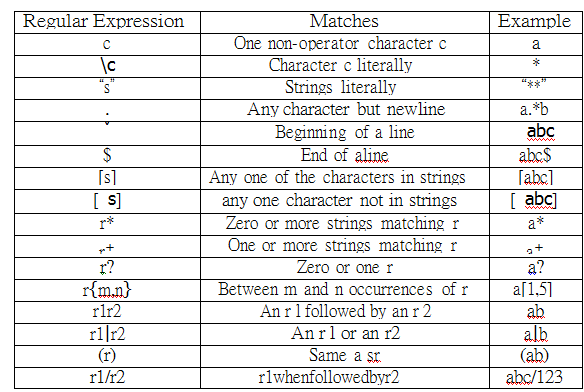
\includegraphics{table.png}
	\end{center}•
	
	\noindent
	Ambiguous Source Rules:\\
	
	Lex can handle ambiguous specifications. When more than one ex-pression can match the current input, Lex choose s as follows:
	\begin{enumerate}
		\item The long est match his preferred.
		\item Am on grules which matched the same number of characters, the rule given first is preferred.
		
	\end{enumerate}•
	
	\noindent
	Built in Functions and variables:\\
	\begin{enumerate}
		\item Int yy lex(void):\\
		Performs lexical analysis on the in put;t his is the primary function generated by the lex utility. The function shall return zero when the end of input is reached; otherwise, it shall return non-zero values (tokens) determined by the actions that are selected.\\
		\item Int yy more(void):\\
		When called, indicates that when the next input string is recog-nized, it is to be appended to the current value of yy text rather than replacing it; the value in yy length all be adjusted accordingly.\\
		\item Int yy less(int n):\\
		Retains n initial characters in yytext, NUL-terminated, and treats
		
	\end{enumerate}•
	
	\noindent
	The remaining characters as if they had not been read; the value in yyleng shall be adjusted accordingly.\\
	
	\noindent
	Int input(void):\\
	Returns the next character from the input, or zero on end-of-file. It shall obtain input from the stream pointer yyin, although possible via an intermediate buffer. Thus, onces can ning has begun, the effect of altering the value of yyin is udefined. The charac-ter reads hall be removed from the input stream of the scanner without any processing by the scanner.\\
	
	\noindent
	Int unput(int c):\\
	Returns the character‘c’to the input; yytext and yylen gareun-defined until then ext expression is matched. The result of using unput() for more characters than have been input is unspecified.\\
	
	\noindent
	Int yywrap(void):\\
	Called by yylex() atend-of-file; the default yywrap() shall always return 1.If the application requires  yylex() to continue processing with another source of input, then the application can include a function yywrap(), which associates another file with the external variable FILE*yyin and shall return a value of zero.\\
	
	\noindent
	int main(int argc,char*argv[]):\\
	Calls yylex()  to perform lexical analysis, thenexits. The user code can contain main() to perform application-specific opera-tions, calling yylex() as applicable.\\
	
	\noindent
	Yyin and yyout:\\
	These are FILE* s to the input and output file respectively. Both are accessible and can be assigned to a value other than stdin and stdout.\\
	
	\noindent
	yytext:\\
	Array of or pointer to char where lex places the current tokens lexeme. The string is automatically null-terminated. It can be modified but not lengthened.\\
	
	\noindent
	yyleng:\\
	Integer that hold sstrlen(yytext).\\
	
	\noindent
	yylineno:\\
	Integer that keeps count of lines read. It is maintained automati-c all y by yylex() for each | nen countered.\\
	
	\noindent
	Example of a lex program:\\
	
	\%{\\
		/* C code to be copied verbatim */ \\
		\#include$<$stdio.h$>$\\
		\%}\\
	
	/*This tells flex to read only one input file*/\\
	\%option no yywrap\\
	
	\%\%\\
	/***Rules section***/\\
	
	/*$[0-9]+matches a string of one or more digits*/[0-9]+$\\
	{\\
		/*yytext is a string containing the matched text.  */printf(“Sawaninteger:\%s”,yytext);\\
	}\\
	{/*Ignore all other characters.*/}\\
	
	\%\%\\
	/***C Code section***/\\
	
	Int main$($void$)$\\
	{\\
		/*Call the lexer, then quit.*/yylex();\\
		return0;\\
	}\\
	
	\noindent
	Usage:\\
	
	There are two steps in compiling a LEX source program. First, the LEX source must be turned into a generated program in the host general purpose language. Then this program must be compiled and loaded, usually with a library of LEX subroutines. The generated program is on a file named lex.yy.c. The I/O library is defined in terms of the C standard library.\\
	
	\noindent
	Command:\\
	
	\$lex$<$programname$>$.l
	\$gcclex.yy.c—ll
	\$./a.out
	
	\noindent
	CONCLUSION :\\
	
	Thus, we have studied Lexical Analyzer for sample language.\\\\\\
	
	\begin{tabular}{|c|c|c|c|c|}
		•$Roll$ $No$ & $Name$ $of$ $Student$ & $Date$ $of$ $performance$ & $Date$ $of$ $Checking$ & $Signature$ $of$ $Staff$ \\ \hline
		•$BECOC357$ & Sunny Shah& 23 / 06 / 2017& 30 / 06 / 2017 &  \\ \hline
	\end{tabular}•
	•
	\newpage
	\section{PLAGARISM REPORT :}
	\begin{figure}[h!]
		\centering
		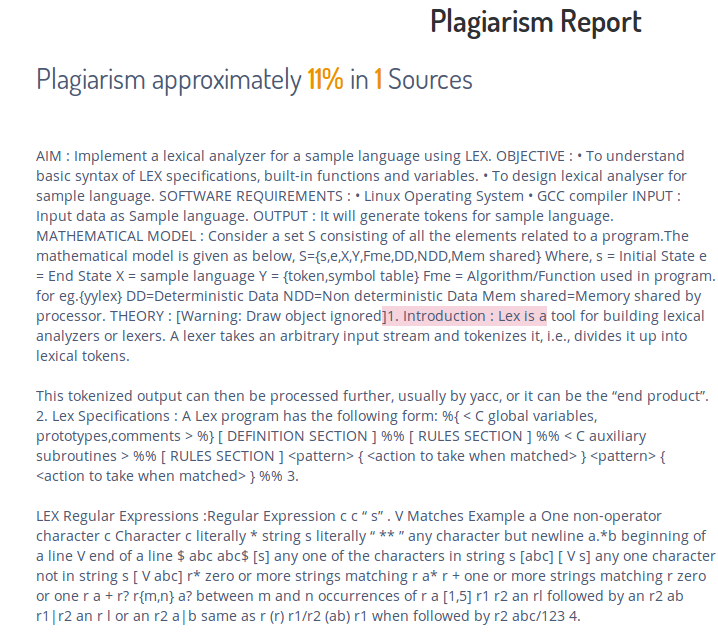
\includegraphics[height=4in,width=4in]{plagiarism1.png}
		\caption{Plagarism Checker: www.smallseotools.com/plagarism-checker}
	\end{figure}
	\newpage
	
\end{document}

